\chapter{Appendix}
  \label{sec:appendix}

  \subsection{Figures}

  \begin{figure}[H]
    \centering
    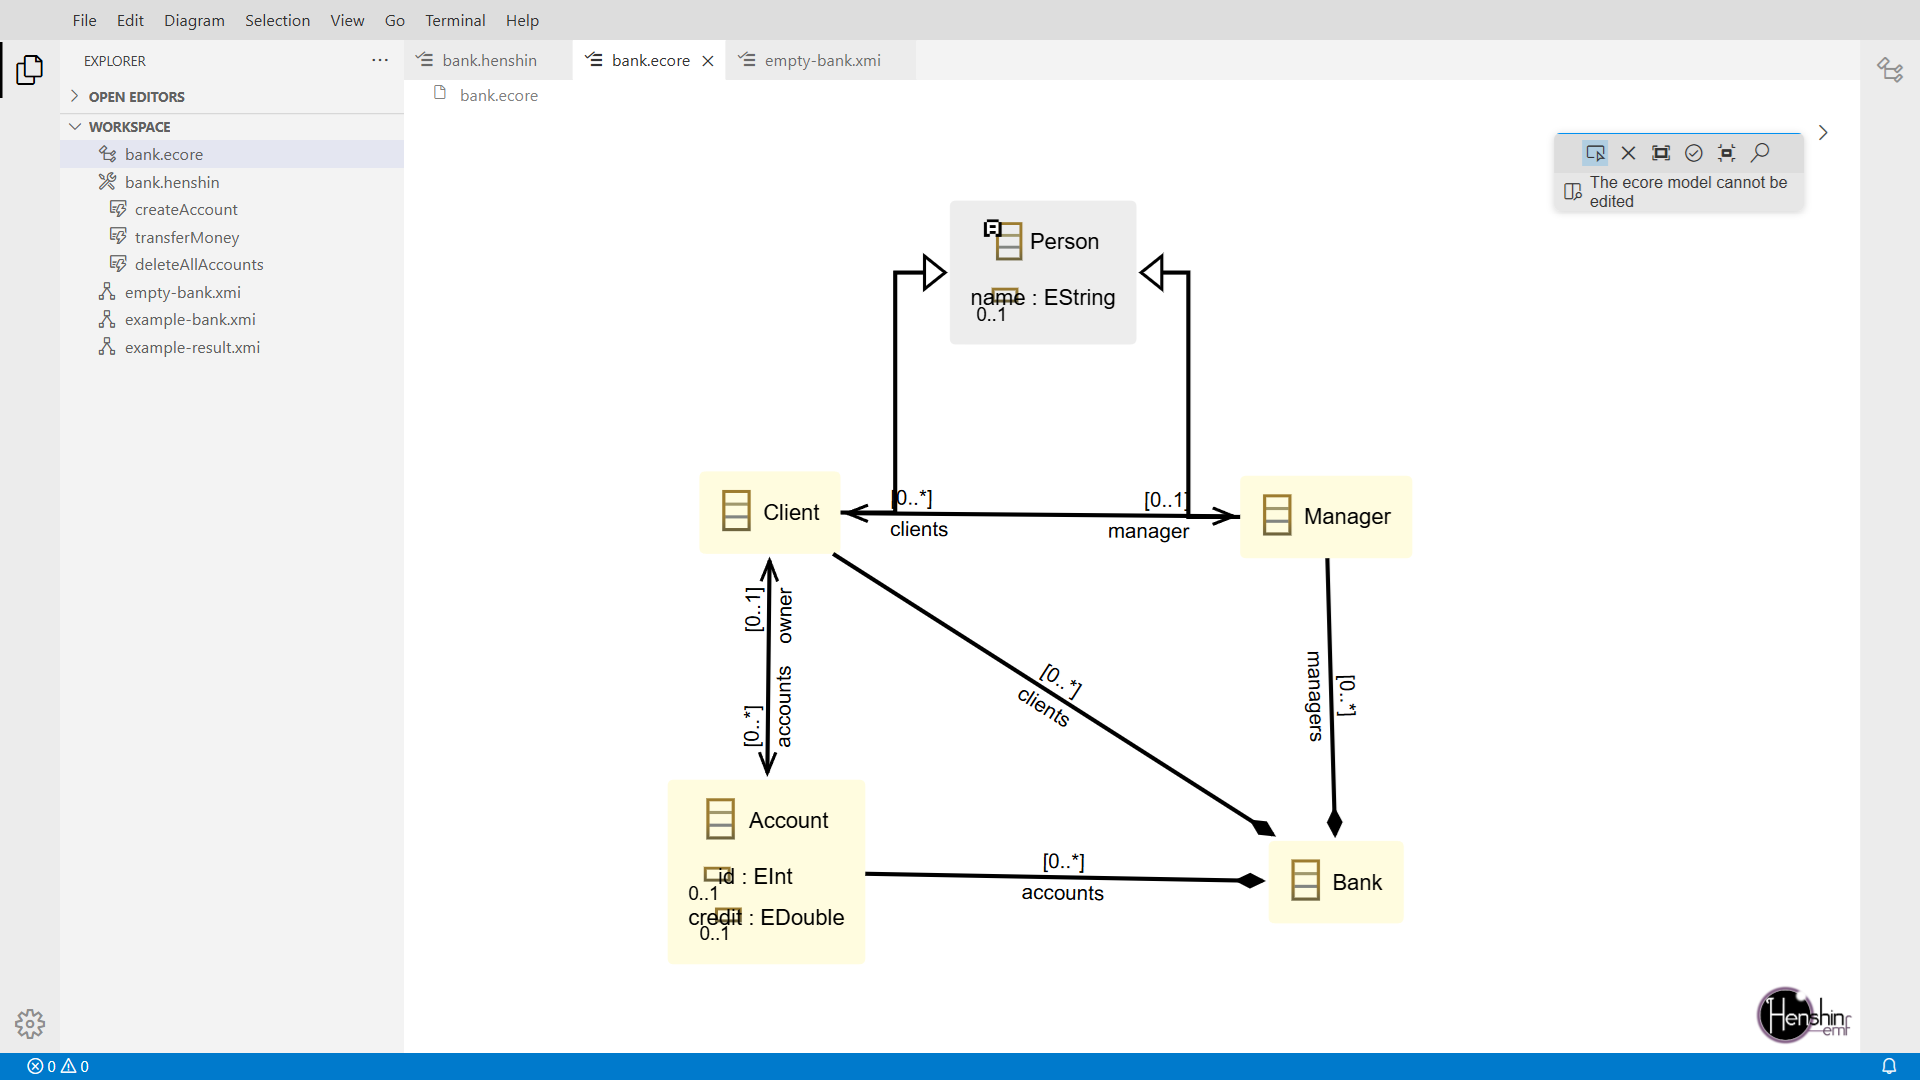
\includegraphics[width=1\textwidth]{ecore-ui}
    \caption{Henshin Web Ecore graph editor}
    \label{fig:ecore-ui}
  \end{figure}

  \begin{figure}[H]
    \centering
    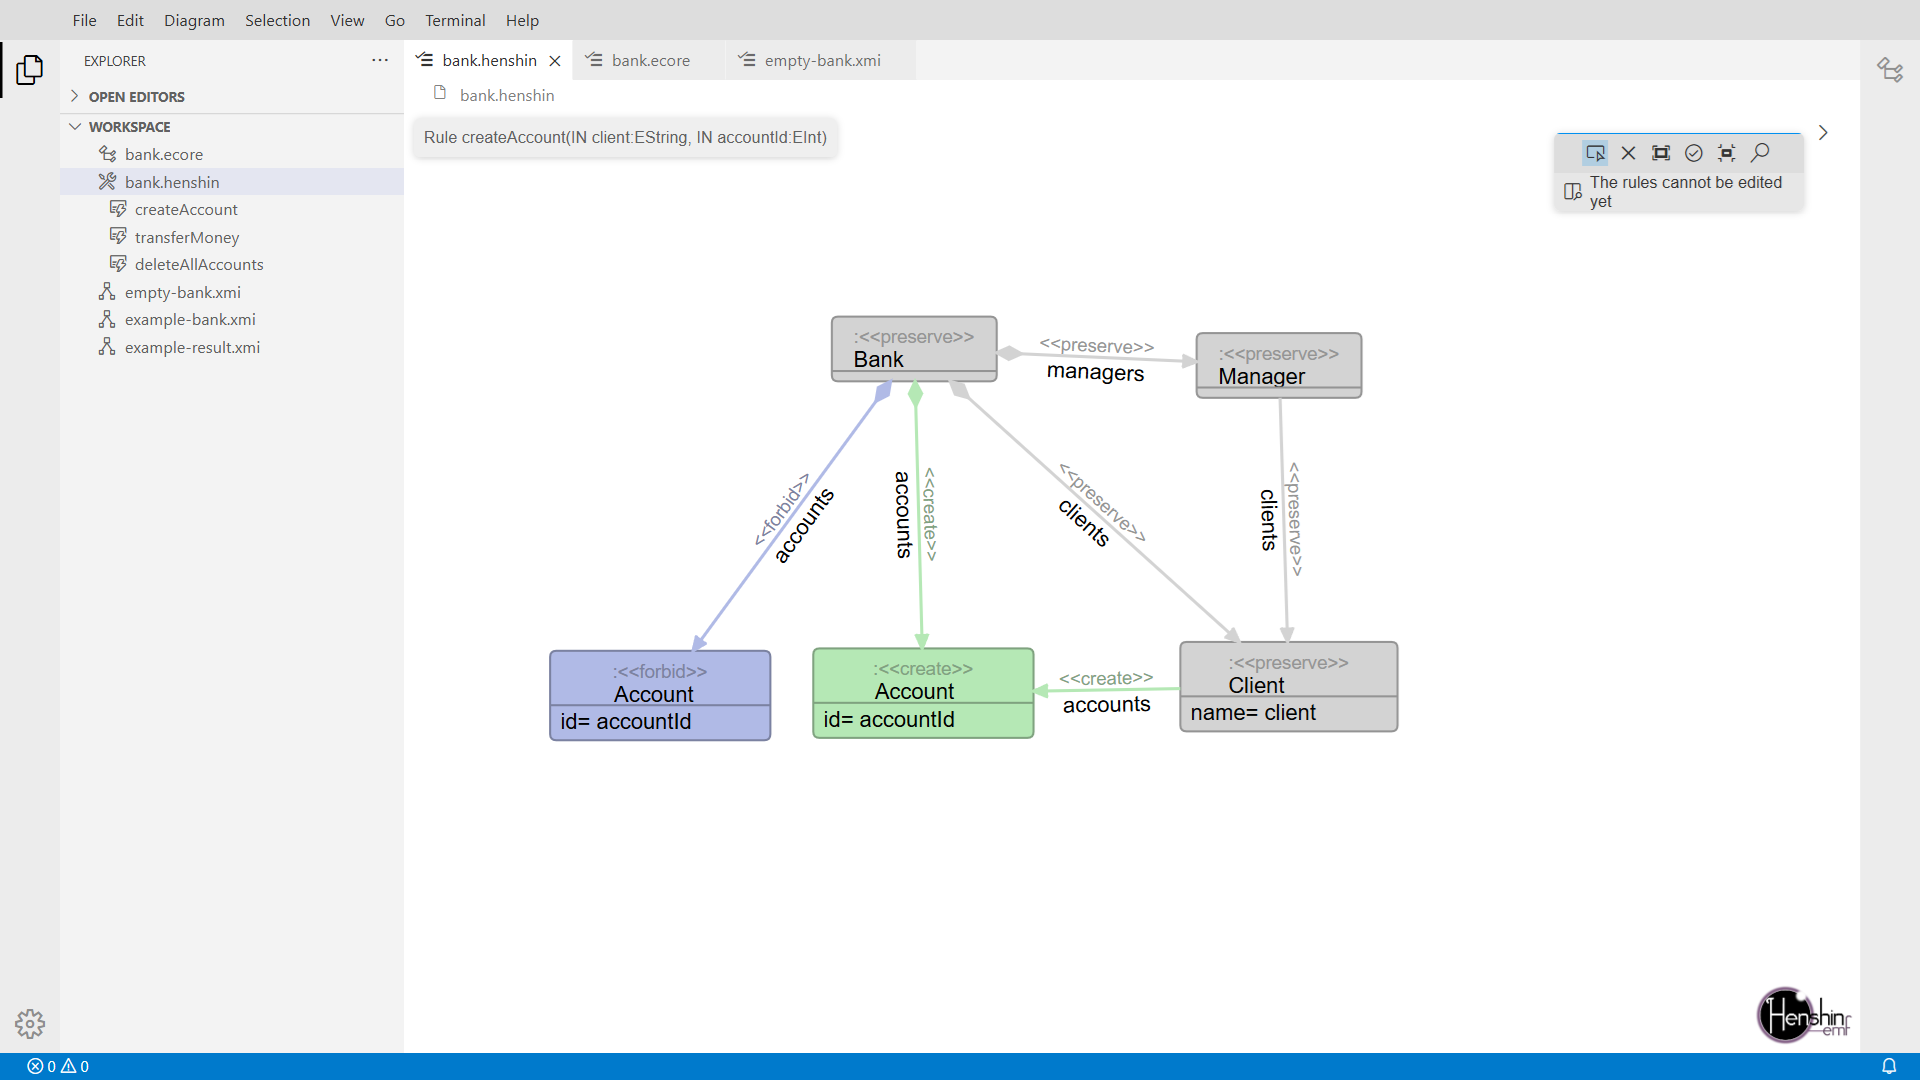
\includegraphics[width=1\textwidth]{rule-ui}
    \caption{Henshin Web Rules graph editor}
    \label{fig:rule-ui}
  \end{figure}

  \begin{figure}[H]
    \centering
    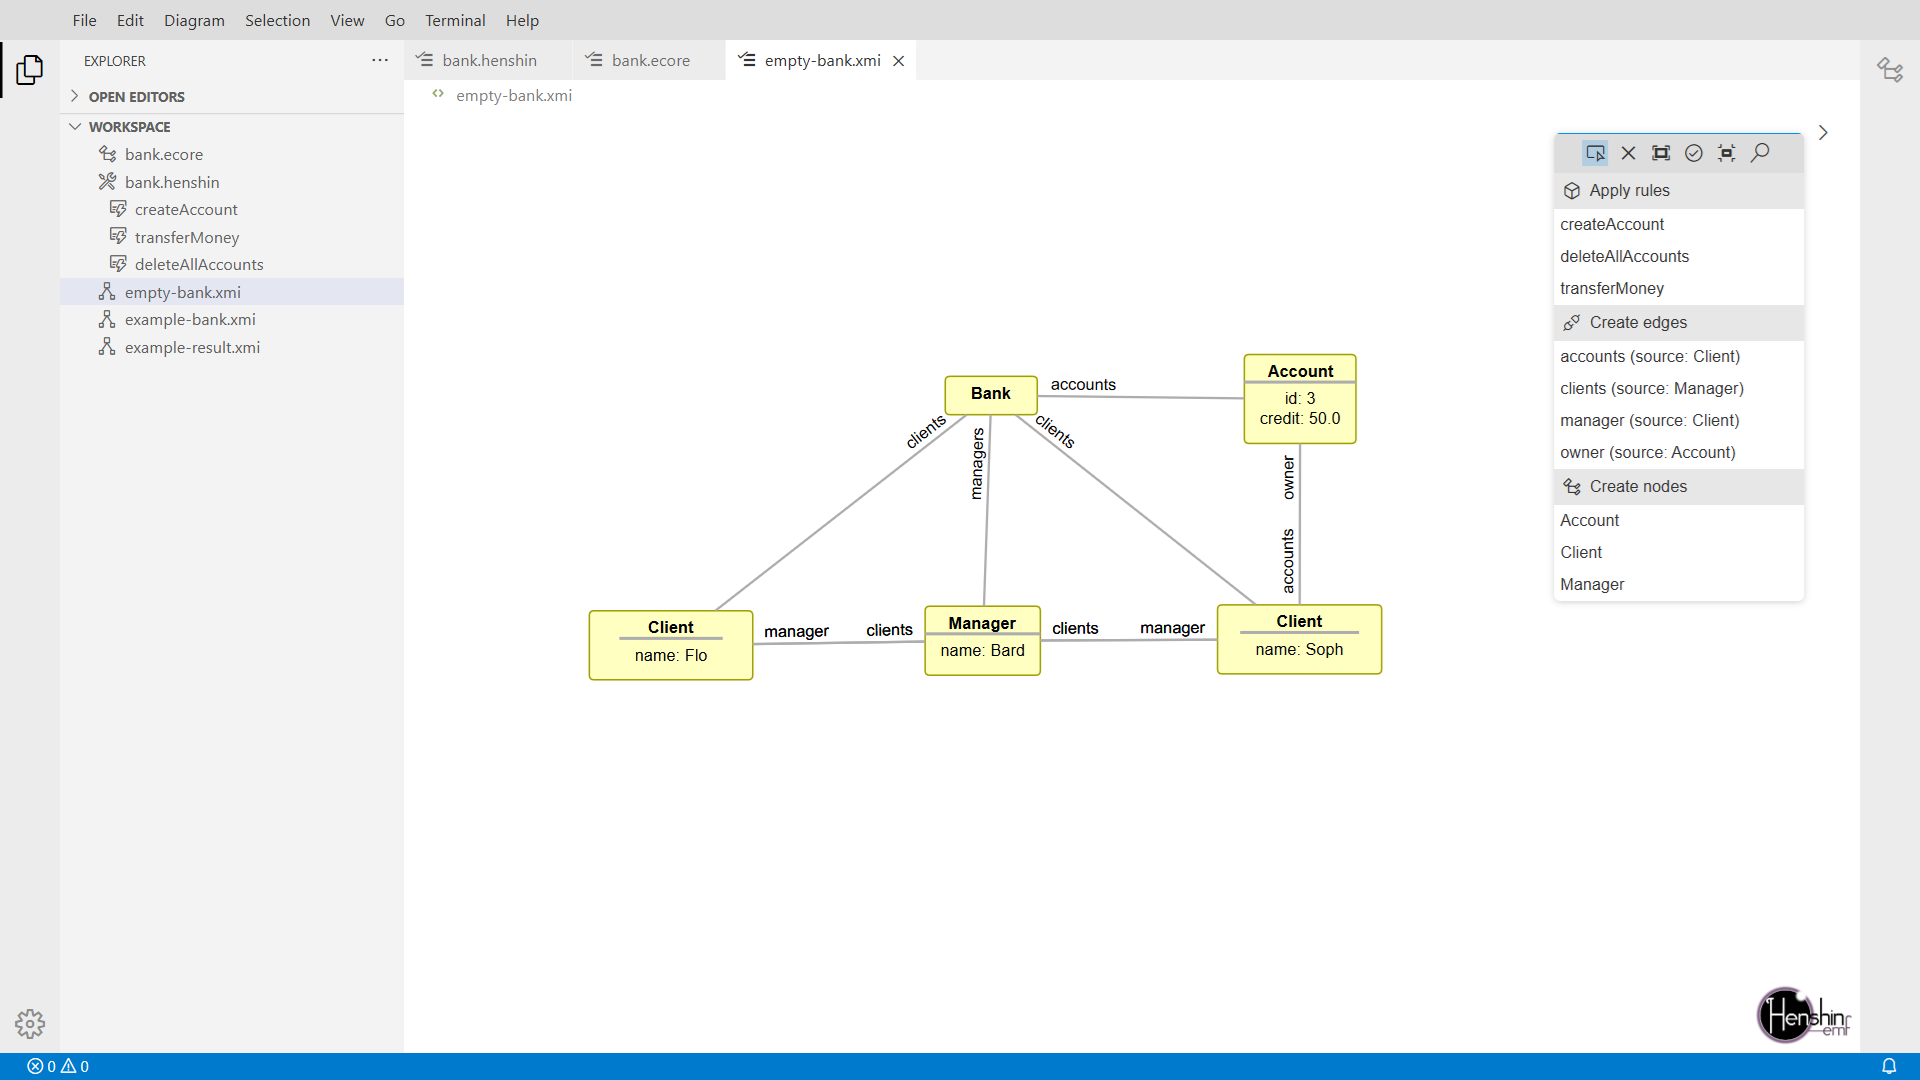
\includegraphics[width=1\textwidth]{xmi-ui}
    \caption{Henshin Web Instance graph editor}
    \label{fig:xmi-ui}
  \end{figure}

  % User Guide
  \begin{figure}[h]
    \centering
    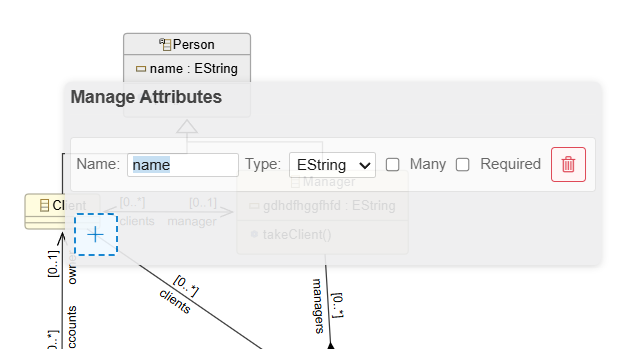
\includegraphics[width=0.7\textwidth]{attribute-editor}
    \caption{Attribute Editor Window}
    \label{fig:attribute-editor}
  \end{figure}
  \begin{figure}[h]
    \centering
    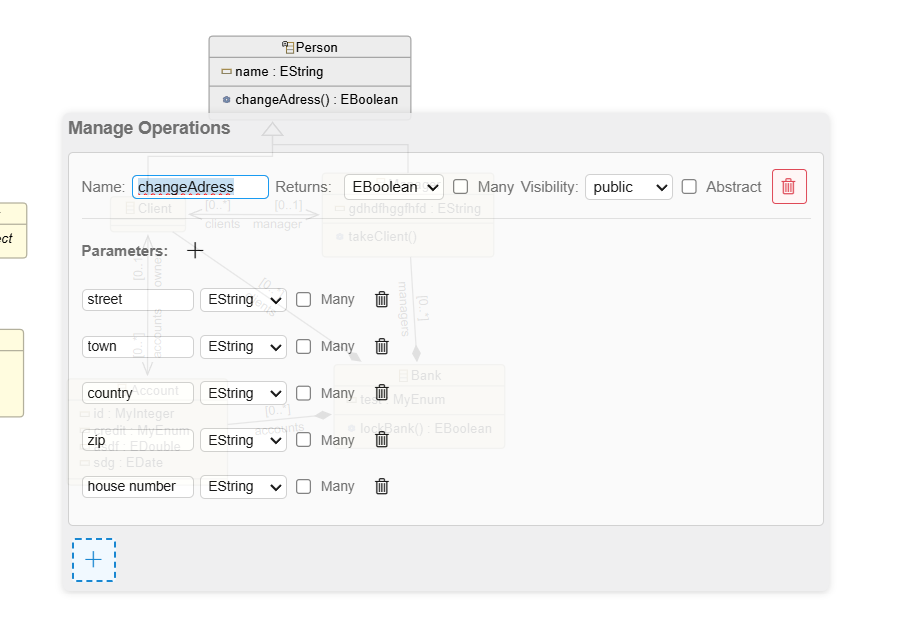
\includegraphics[width=0.7\textwidth]{operation-editor}
    \caption{Operation Editor Window}
    \label{fig:operation-editor}
  \end{figure}
  \begin{figure}[h]
    \centering
    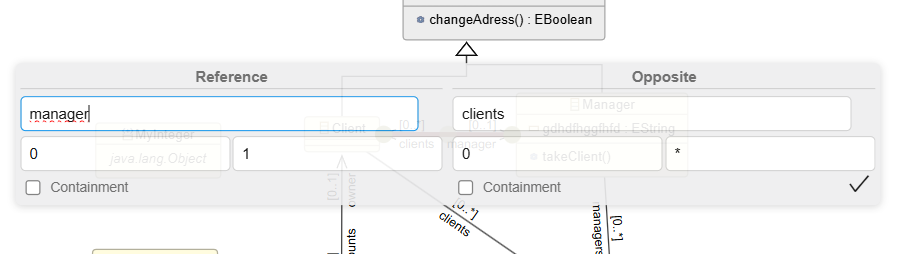
\includegraphics[width=0.7\textwidth]{reference-editor}
    \caption{Reference Editor Window}
    \label{fig:reference-editor}
  \end{figure}
  \begin{figure}[h]
    \centering
    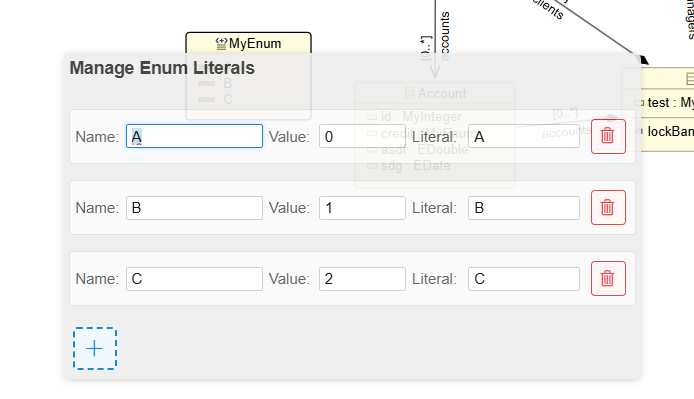
\includegraphics[width=0.7\textwidth]{enum-editor}
    \caption{Enum Editor Window}
    \label{fig:enum-editor}
  \end{figure}
    \begin{figure}[h]
    \centering
    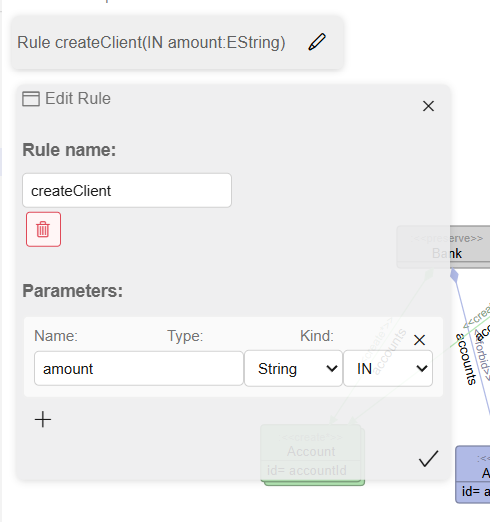
\includegraphics[width=0.7\textwidth]{rule-editor}
    \caption{Rule Editor Window}
    \label{fig:rule-editor}
  \end{figure}
      \begin{figure}[h]
    \centering
    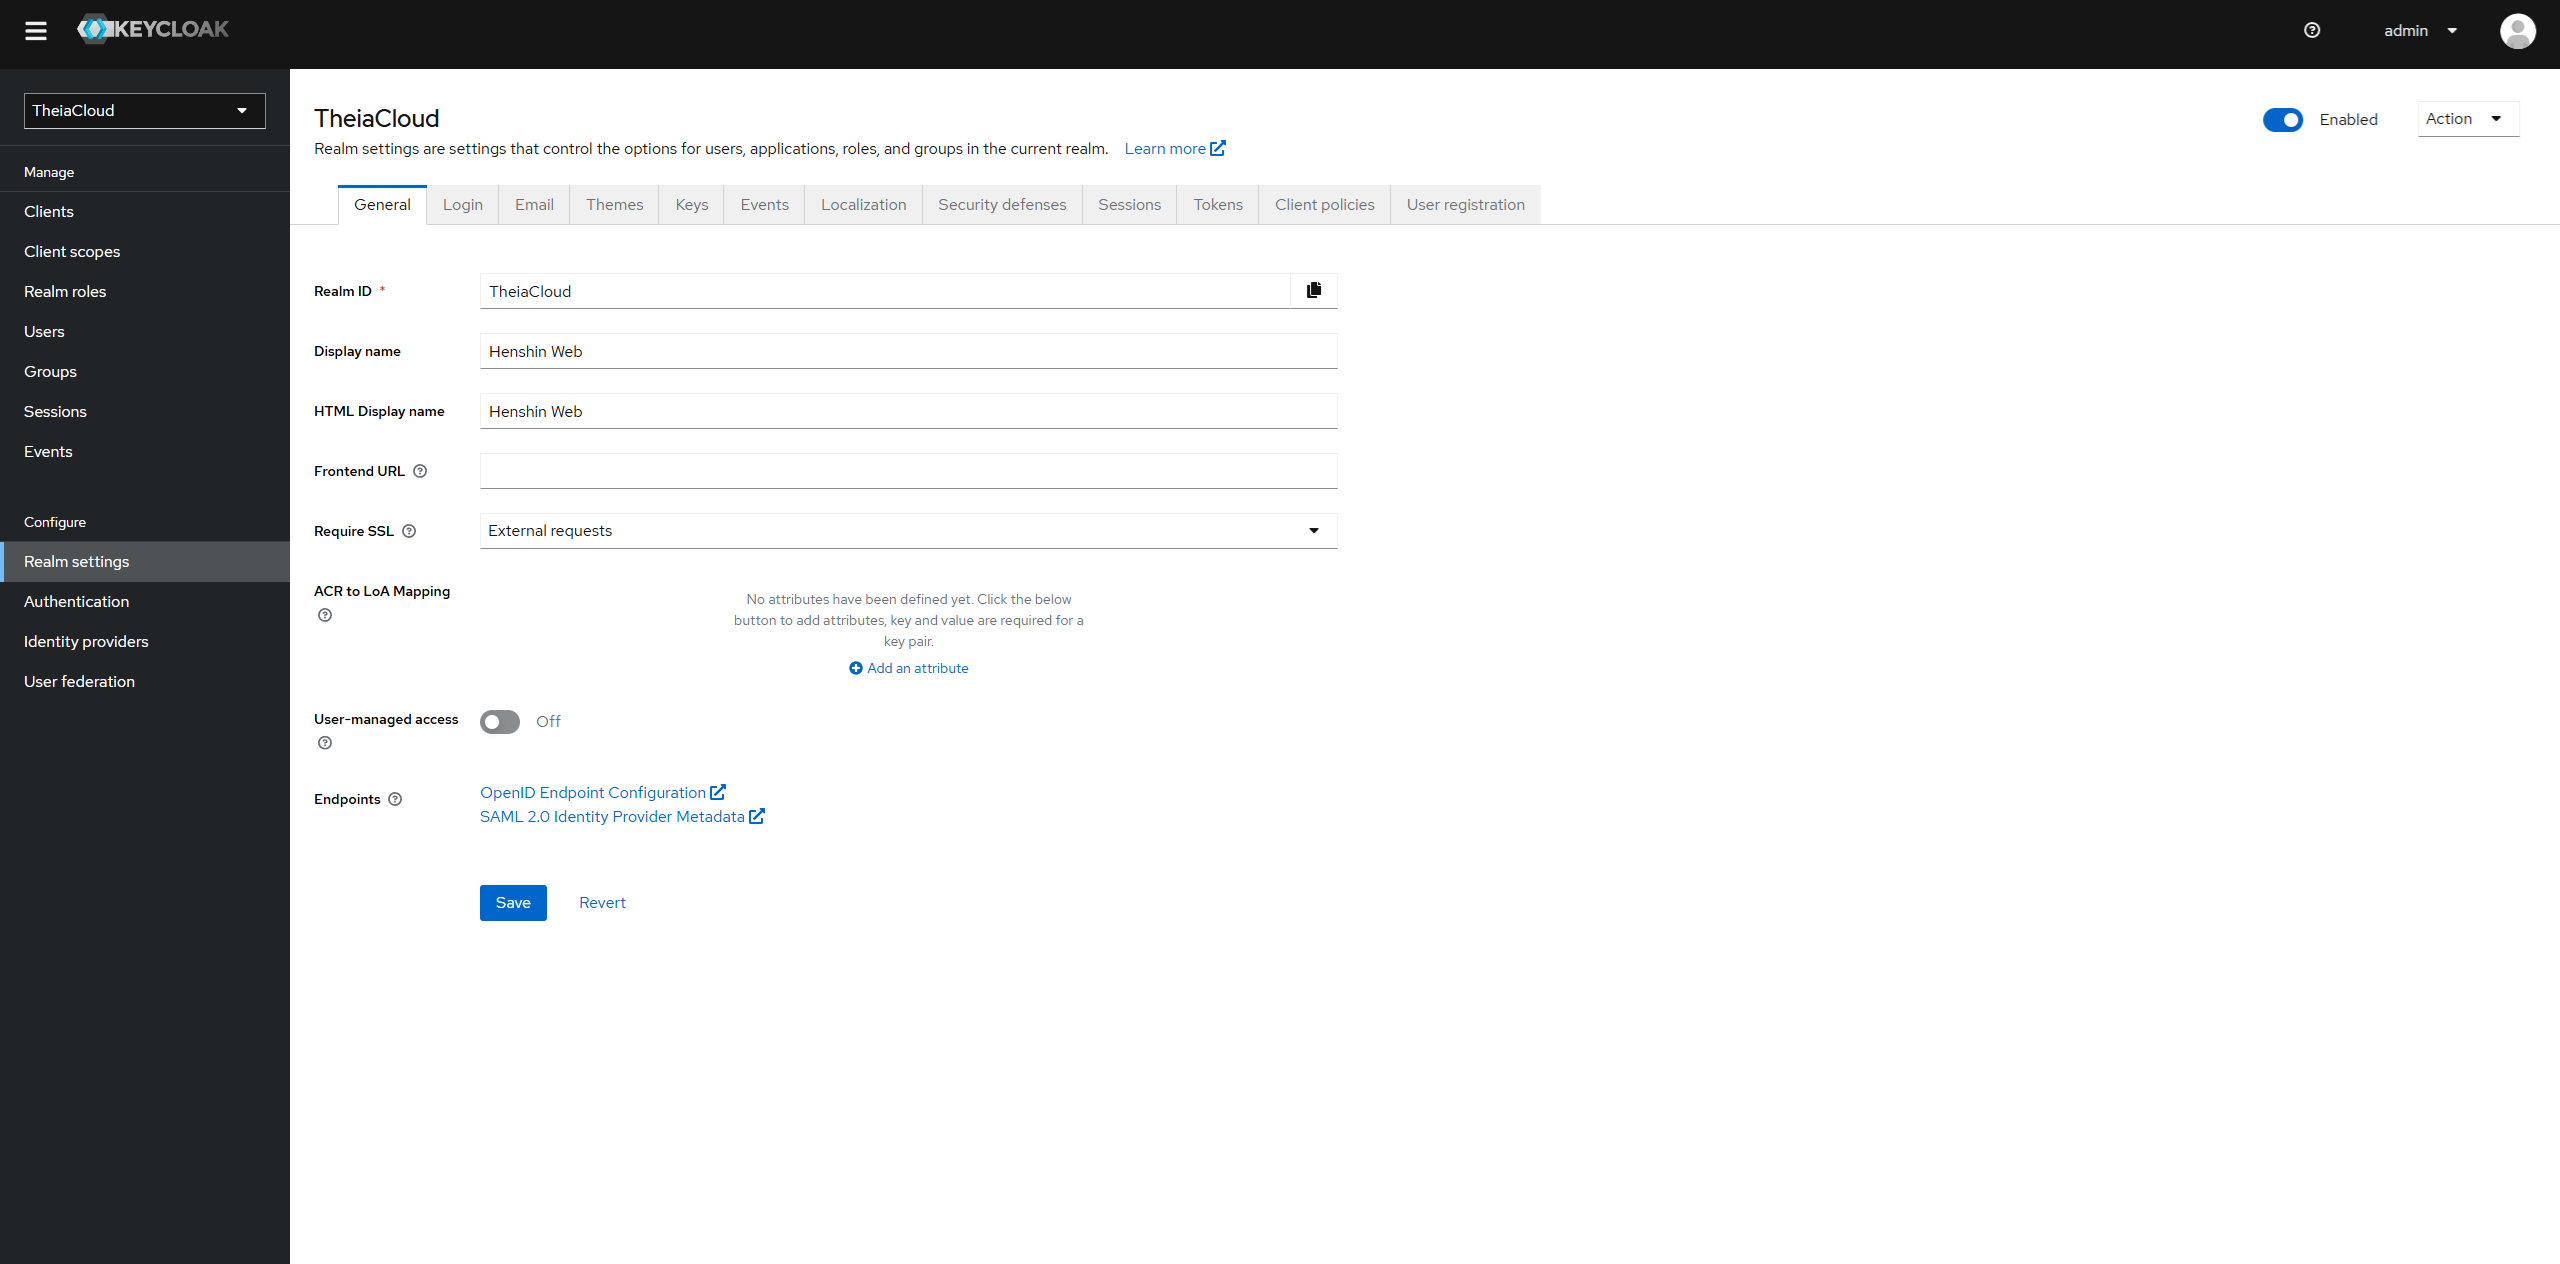
\includegraphics[width=0.7\textwidth]{admin-console}
    \caption{Keycloak Admin Console}
    \label{fig:admin-console}
  \end{figure}



  \subsection{Code Listings}

    % \begin{lstlisting}[language=Java, caption={Parts of \code{NotationAdapter}}, label={lst:notation-adapter}]
public class NotationAdapter extends AdapterImpl {
    private Shape shape;

    public NotationAdapter(Shape shape) {
        this.shape = shape;
    }

    @Override
    public boolean isAdapterForType(Object type) {
        return type == NotationAdapter.class;
    }

    public static Shape getOrAssignNotation(DynamicEObjectImpl obj) {
        // Return existing Notation if present
        for (var adapter : obj.eAdapters()) {
            if (adapter instanceof NotationAdapter) {
                return ((NotationAdapter) adapter).getShape();
            }
        }

        // Assign new Notation
        String hashId = hashENodeObject(obj);
        Shape shape = notationMap.get(hashId);
        if(shape == null) {
            shape = XMINotationFactory.createNewShape(obj);
        }
        NotationAdapter newAdapter = new NotationAdapter(shape);
        obj.eAdapters().add(newAdapter);

        return shape;
    }

    public static String hashENodeObject(DynamicEObjectImpl eObject) {
        StringBuilder result = new StringBuilder();

        result.append(eObject.eClass().getName()).append(":");
        result.append(DynamicEObjectImpl.class.getSimpleName());

        for (EStructuralFeature feature : eObject.eClass().getEAllStructuralFeatures()) {
            if (feature instanceof EAttribute) {
                result.append("-").append(feature.getName());
                result.append(":").append(feature.getEType().getName());
                result.append("=").append(eObject.eGet(feature).toString());
            }
        }

        return result.toString();
    }

    public static void dispose() {
        notationMap.clear();
    }
}
\end{lstlisting}

    % \begin{lstlisting}[language=Java, caption={Parts of \code{XMIGModelFactory}}, label={lst:gmodel-factory}]
@Override
protected void fillRootElement(GModelRoot newRoot) {
    EGraph instanceNodes = modelState.getInstanceGraph();

    newRoot.getChildren().addAll(instanceNodes.stream()
            .map(eObject -> (DynamicEObjectImpl) eObject) //
            .map(this::createNode)//
            .toList());

    ...
}

public GNode createNode(DynamicEObjectImpl eObject) {
    String type = DefaultTypes.NODE;
    if(eObject.eContainer() == null) {
        type = HenshinTypes.XMI_ROOT_NODE;
    }

    GNodeBuilder b = new GNodeBuilder(type) //
            .id(UUIDAdapter.getOrAssignId(eObject)) //
            .layout(GConstants.Layout.VBOX) //
            .addCssClass(HenshinCss.XMI_NODE) //
            .addArguments(GArguments.cornerRadius(3))
            .add(buildHeader(eObject));
    if(!eObject.eClass().getEAllAttributes().isEmpty()) {
        b.add(createAttributesCompartment(eObject.eClass().getEAllAttributes(), eObject));
    }
    applyShapeData(eObject,b);
    return b.build();
}

private GLabel buildHeader(EObject eObject) {
    return new GLabelBuilder(DefaultTypes.LABEL) //
            .id(UUIDAdapter.toLabelId(eObject))
            .addCssClass(HenshinCss.XMI_LABEL)
            .text(eObject.eClass().getName()) //
            .build();
}

...
\end{lstlisting}

    % Define Docker language for listings
\lstdefinelanguage{Docker}{
  morekeywords={FROM, RUN, CMD, LABEL, EXPOSE, ENV, ADD, COPY, ENTRYPOINT, VOLUME, USER, WORKDIR, ARG, ONBUILD, STOPSIGNAL, HEALTHCHECK, SHELL},
  morecomment=[l]{\#},
  morestring=[b]",
  morestring=[b]',
}

\begin{lstlisting}[language=Docker, caption={Dockerfile for Henshin Web Model Transformation Application}, label={lst:dockerfile}]
# Setup dev environment
FROM node:18-bullseye AS build

ENV DEBIAN_FRONTEND=noninteractive

RUN apt-get update && apt-get install -y --no-install-recommends \
    git \
    bash \
    maven \
    openjdk-17-jdk \
    software-properties-common \
    libxkbfile-dev \
    libsecret-1-dev \
    build-essential \
    libssl-dev \
    && rm -rf /var/lib/apt/lists/*


# Build the Java backend
FROM build AS backend

WORKDIR /henshin-editor

COPY ./src/glsp-server ./glsp-server

WORKDIR /henshin-editor/glsp-server

# Copy Maven settings for GitLab authentication
COPY ./src/glsp-server/.m2/settings.xml /root/.m2/settings.xml

# Verify settings file exists and run Maven with explicit settings
RUN mvn clean verify -s /root/.m2/settings.xml

# Build frontend
FROM build AS frontend

WORKDIR /henshin-editor

COPY ./src/glsp-client ./glsp-client

WORKDIR /henshin-editor/glsp-client

RUN yarn install && \
    yarn build

WORKDIR /henshin-editor
COPY --from=backend /henshin-editor/glsp-server ./glsp-server
WORKDIR /henshin-editor/glsp-client

# Create plugins directory for Theia (even if empty)
RUN mkdir -p henshin-browser-app/plugins

RUN yarn autoclean --init && \
    echo *.ts >> .yarnclean && \
    echo *.ts.map >> .yarnclean && \
    echo *.spec.* >> .yarnclean && \
    yarn autoclean --force && \
    yarn cache clean


# Build production image
FROM node:18-bullseye-slim AS production
ENV DEBIAN_FRONTEND=noninteractive

# Theia dependencies/Java
RUN apt-get update && apt-get install -y --no-install-recommends \
    software-properties-common \
    libxkbfile-dev \
    libsecret-1-dev \
    ca-certificates-java \
    openjdk-17-jdk \
    build-essential \
    libssl-dev \
    wget \
    gnupg \
    git \
    gdb \
    && rm -rf /var/lib/apt/lists/*

# C/C++ dependencies
RUN add-apt-repository 'deb http://apt.llvm.org/bullseye/ llvm-toolchain-bullseye-14 main'
RUN wget -O - https://apt.llvm.org/llvm-snapshot.gpg.key | apt-key add -
RUN apt-get update && \
    apt-get -y install clangd-14 cmake && \
    apt-get purge -y && \
    apt-get clean && \
    rm -rf /var/lib/apt/lists/*
RUN update-alternatives --install /usr/bin/clangd clangd /usr/bin/clangd-14 100

# Make readable for root only
RUN chmod -R 750 /var/run/

RUN rm -f /root/.m2/settings.xml

# Create a non-root user with a fixed user id and setup the environment (following Theia Cloud standard)
RUN adduser --system --group --uid 200 theia && \
    chmod g+rw /home && \
    mkdir -p /home/theia && \
    chown -R theia:theia /home/theia
ENV HOME=/home/theia

# Copy frontend from build-stage
WORKDIR /home/theia
COPY --chown=theia:theia --from=frontend /henshin-editor/glsp-client ./glsp-client

# Copy model to production stage (for model comparison)
COPY --from=backend /henshin-editor/glsp-server/target/*.jar \
    /home/theia/glsp-server/target/

# Copy favicon
RUN cp ./glsp-client/henshin-browser-app/favicon.ico ./glsp-client/henshin-browser-app/src-gen/frontend/
RUN sed -i 's/<\/head>/<link rel="icon" href="favicon.ico" \/><\/head>/g' glsp-client/henshin-browser-app/src-gen/frontend/index.html

# Create and setup the persisted project directory
RUN mkdir -p /home/project/persisted/workspace && \
    chown -R theia:theia /home/project && \
    chmod -R 755 /home/project

# Copy workspace content to the persisted location as well
COPY --chown=theia:theia ./src/glsp-client/workspace/ /home/project/persisted/workspace

EXPOSE 3000
USER theia
WORKDIR /home/theia/glsp-client/henshin-browser-app/

ENTRYPOINT [ "node", "/home/theia/glsp-client/henshin-browser-app/src-gen/backend/main.js" ]
CMD [ "--root-dir=/home/project/persisted/workspace", "--hostname=0.0.0.0", "--port=3000", "--plugins=local-dir:/home/theia/glsp-client/henshin-browser-app/plugins", "--build-id=2025-08-11-v2" ]
\end{lstlisting}


